\begin{landscape}
\begin{figure}[htb]\begin{center}
\vskip-1.5cm
\resizebox{1.5\textwidth}{!}{
	\subfigure[]{
          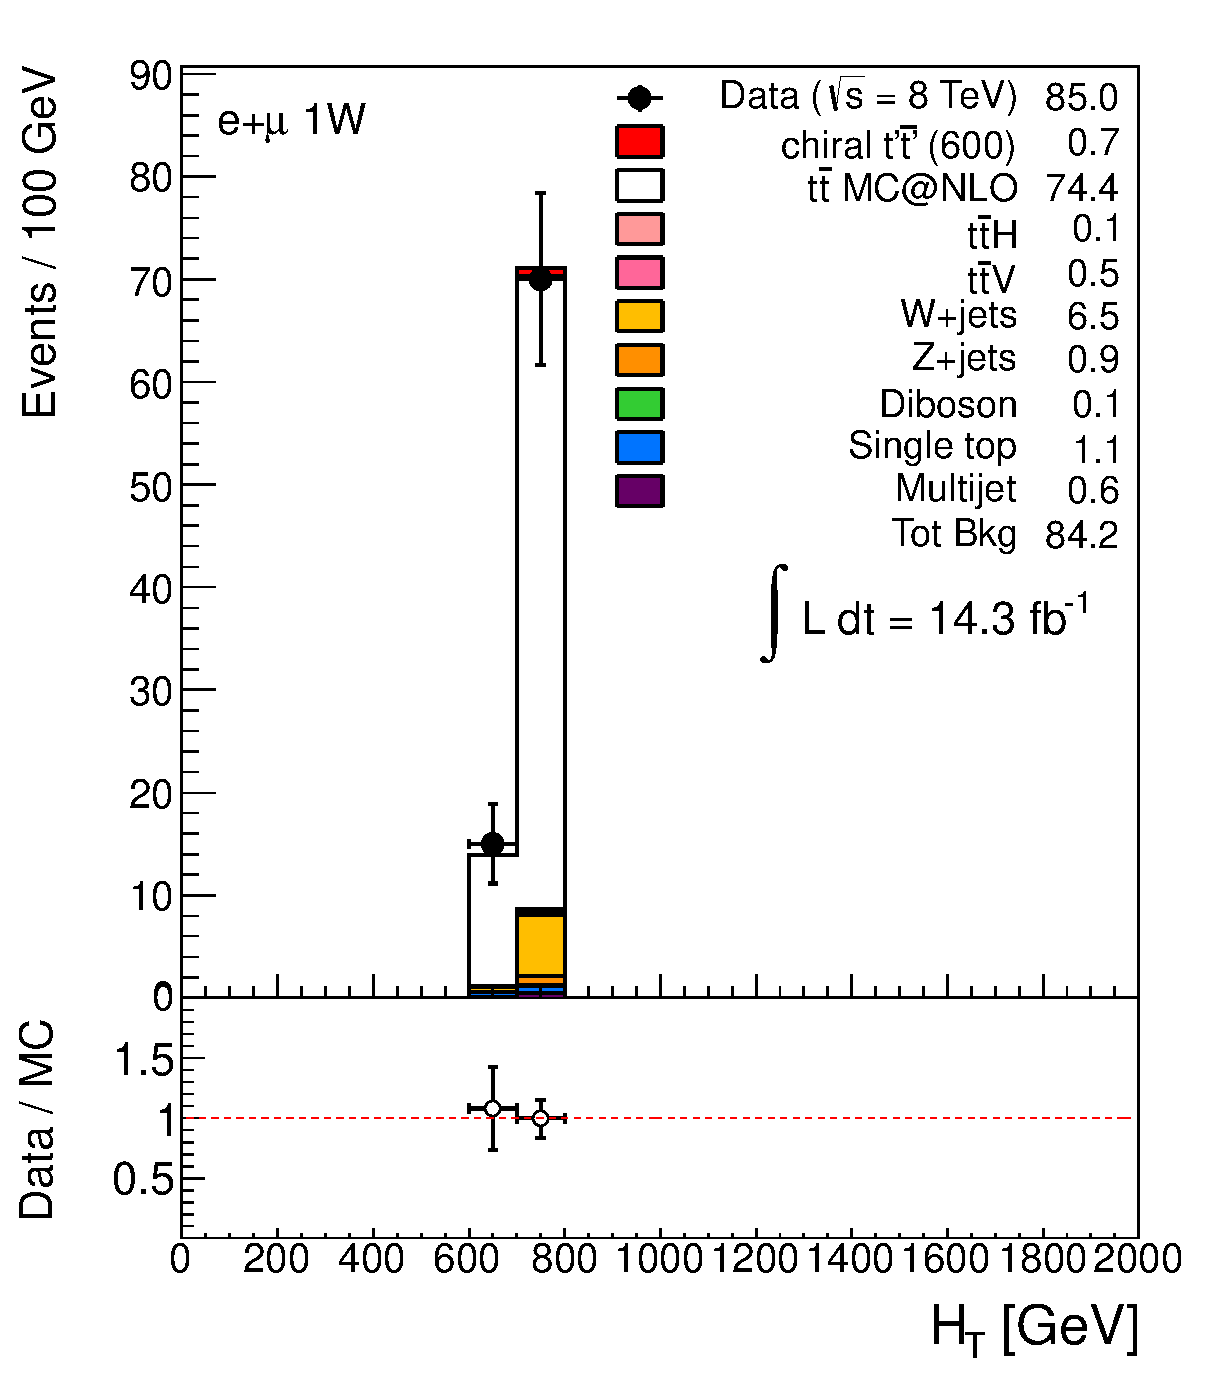
\includegraphics[width=0.3\textwidth]{appendices/figures/genmod/ttbar5200/HTAll_ELEMUONCR1_1W_NOMINAL.eps}}
	\subfigure[]{
          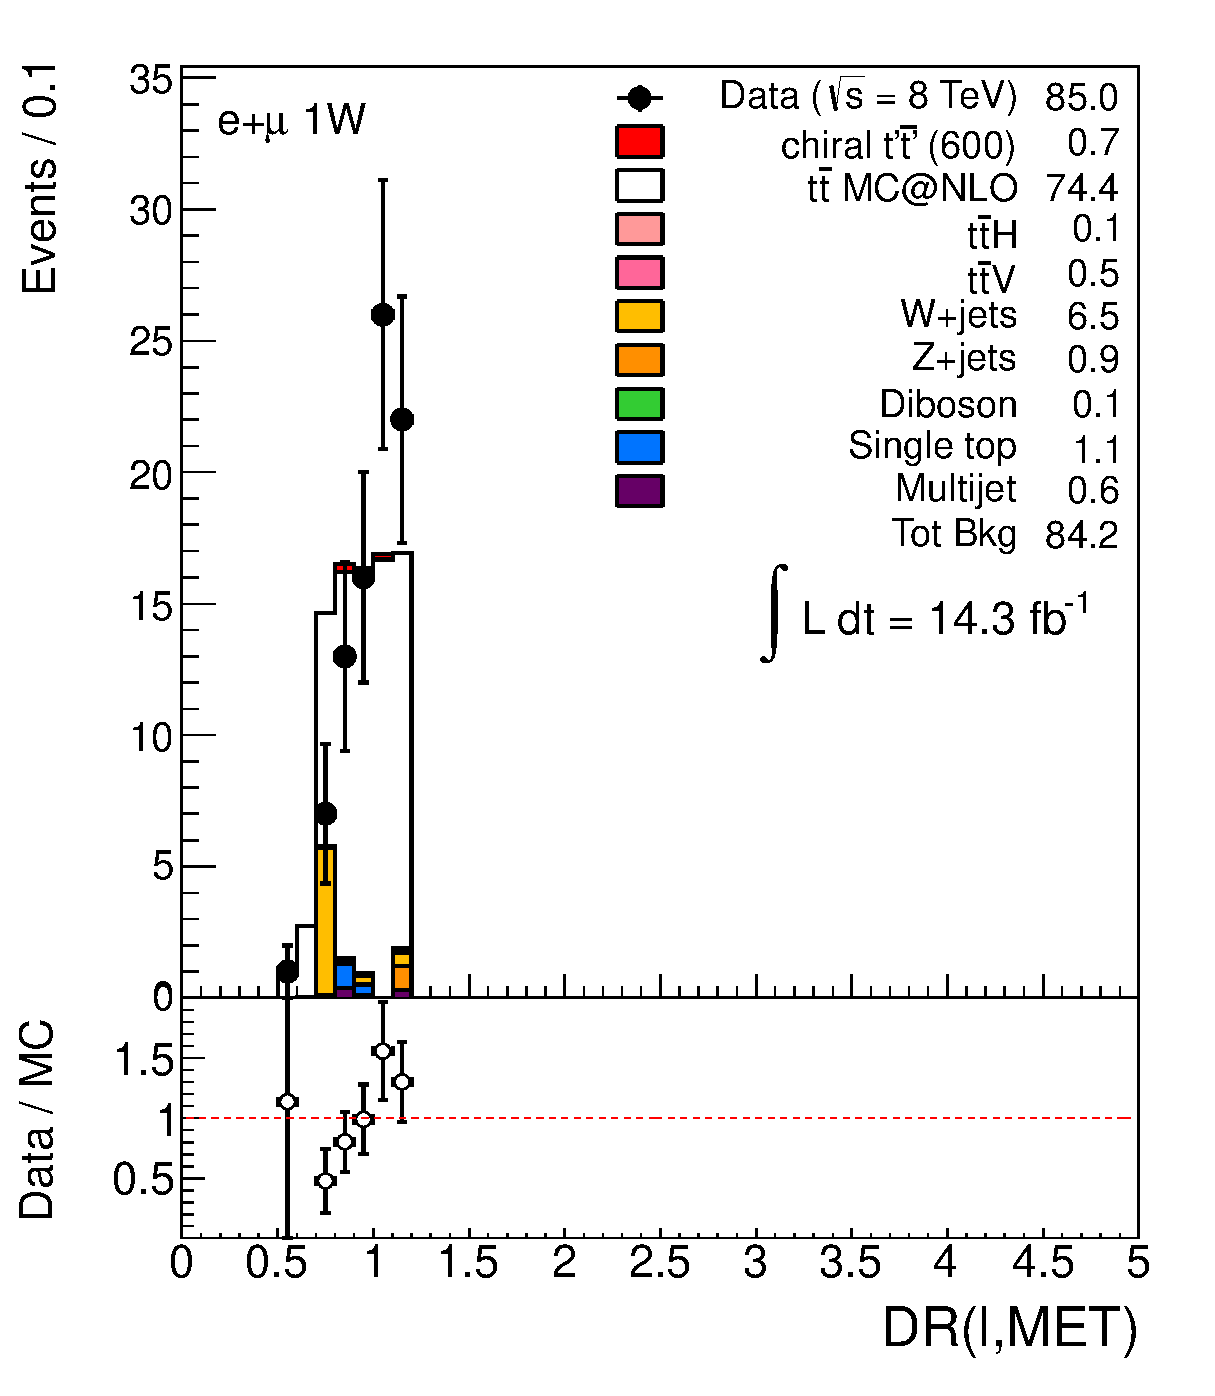
\includegraphics[width=0.3\textwidth]{appendices/figures/genmod/ttbar5200/VLQAna_WbX_DRLepMet_ELEMUONCR1_1W_NOMINAL.eps}}
	\subfigure[]{
          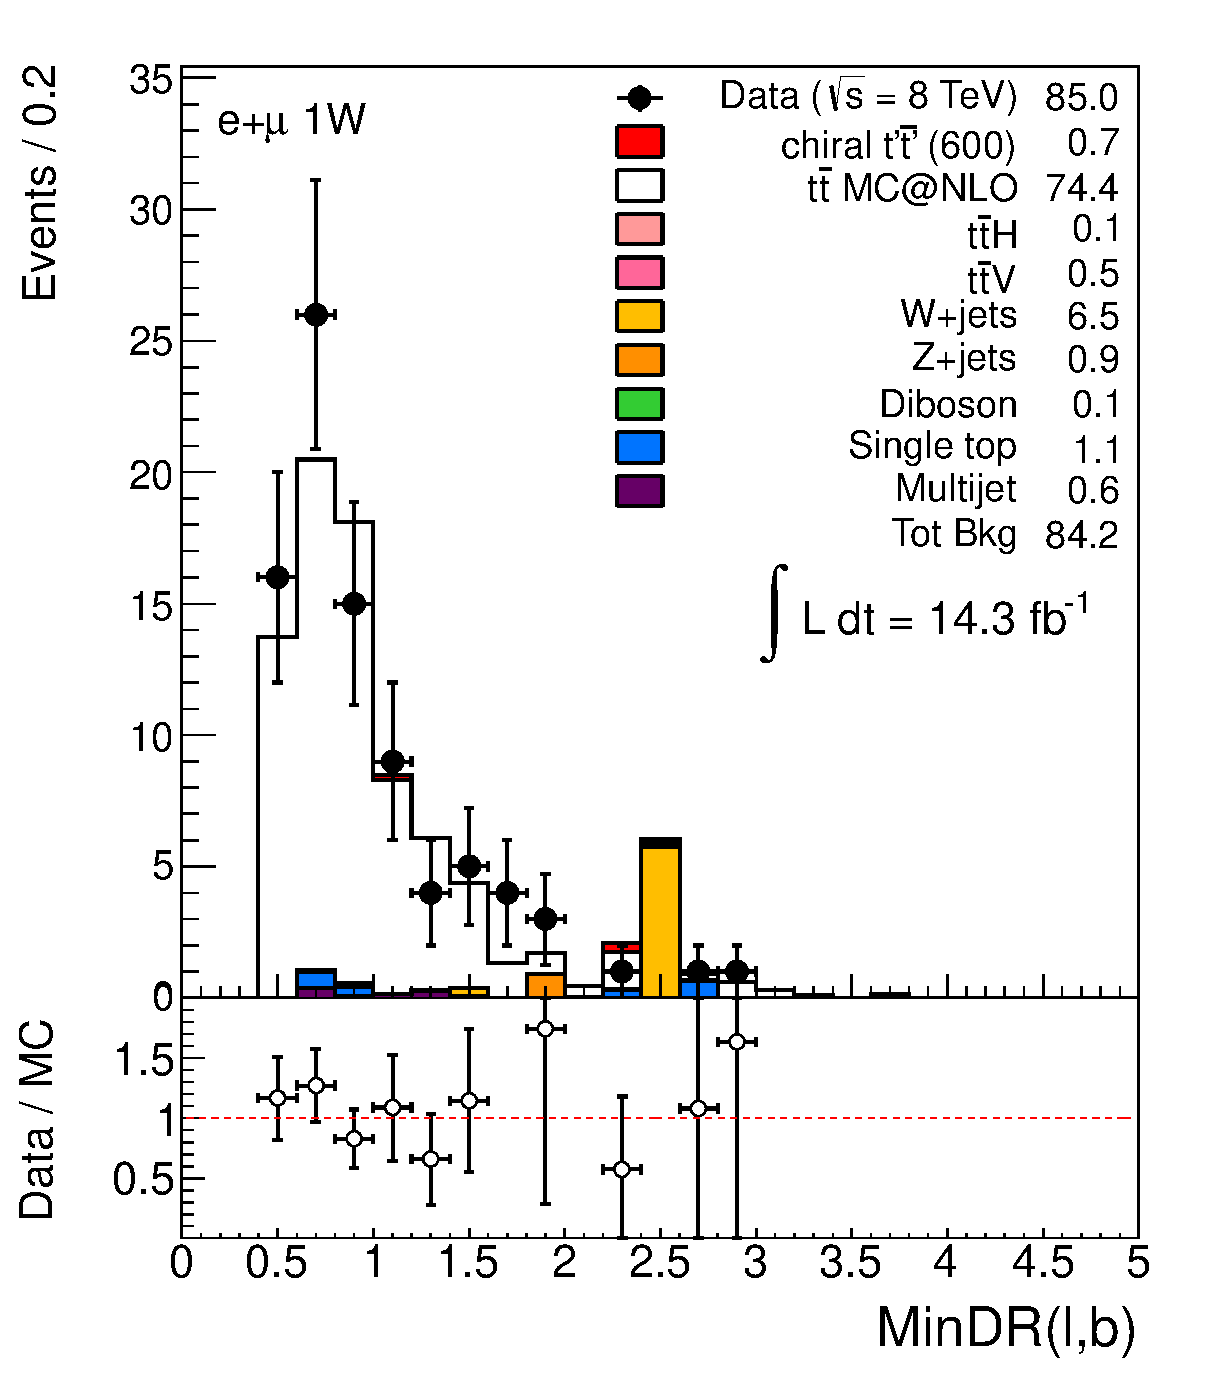
\includegraphics[width=0.3\textwidth]{appendices/figures/genmod/ttbar5200/VLQAna_WbX_MinDRlb_ELEMUONCR1_1W_NOMINAL.eps}}
	\subfigure[]{
          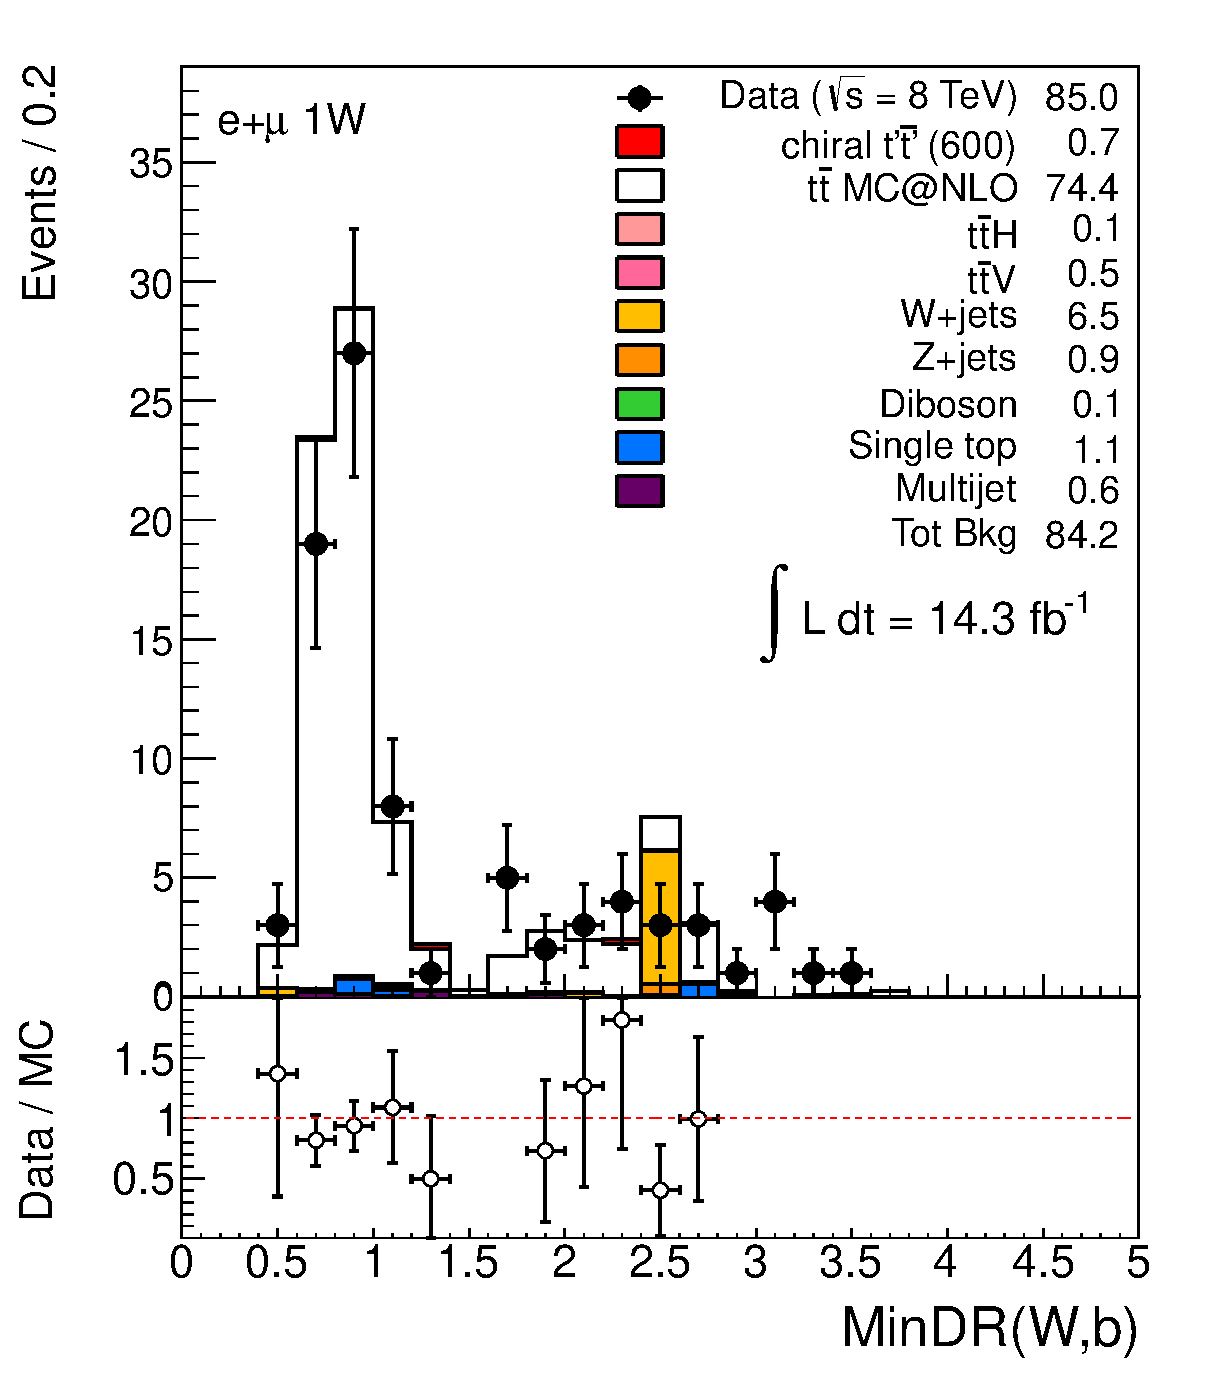
\includegraphics[width=0.3\textwidth]{appendices/figures/genmod/ttbar5200/VLQAna_WbX_MinDRWb_ELEMUONCR1_1W_NOMINAL.eps}}
	\subfigure[]{
          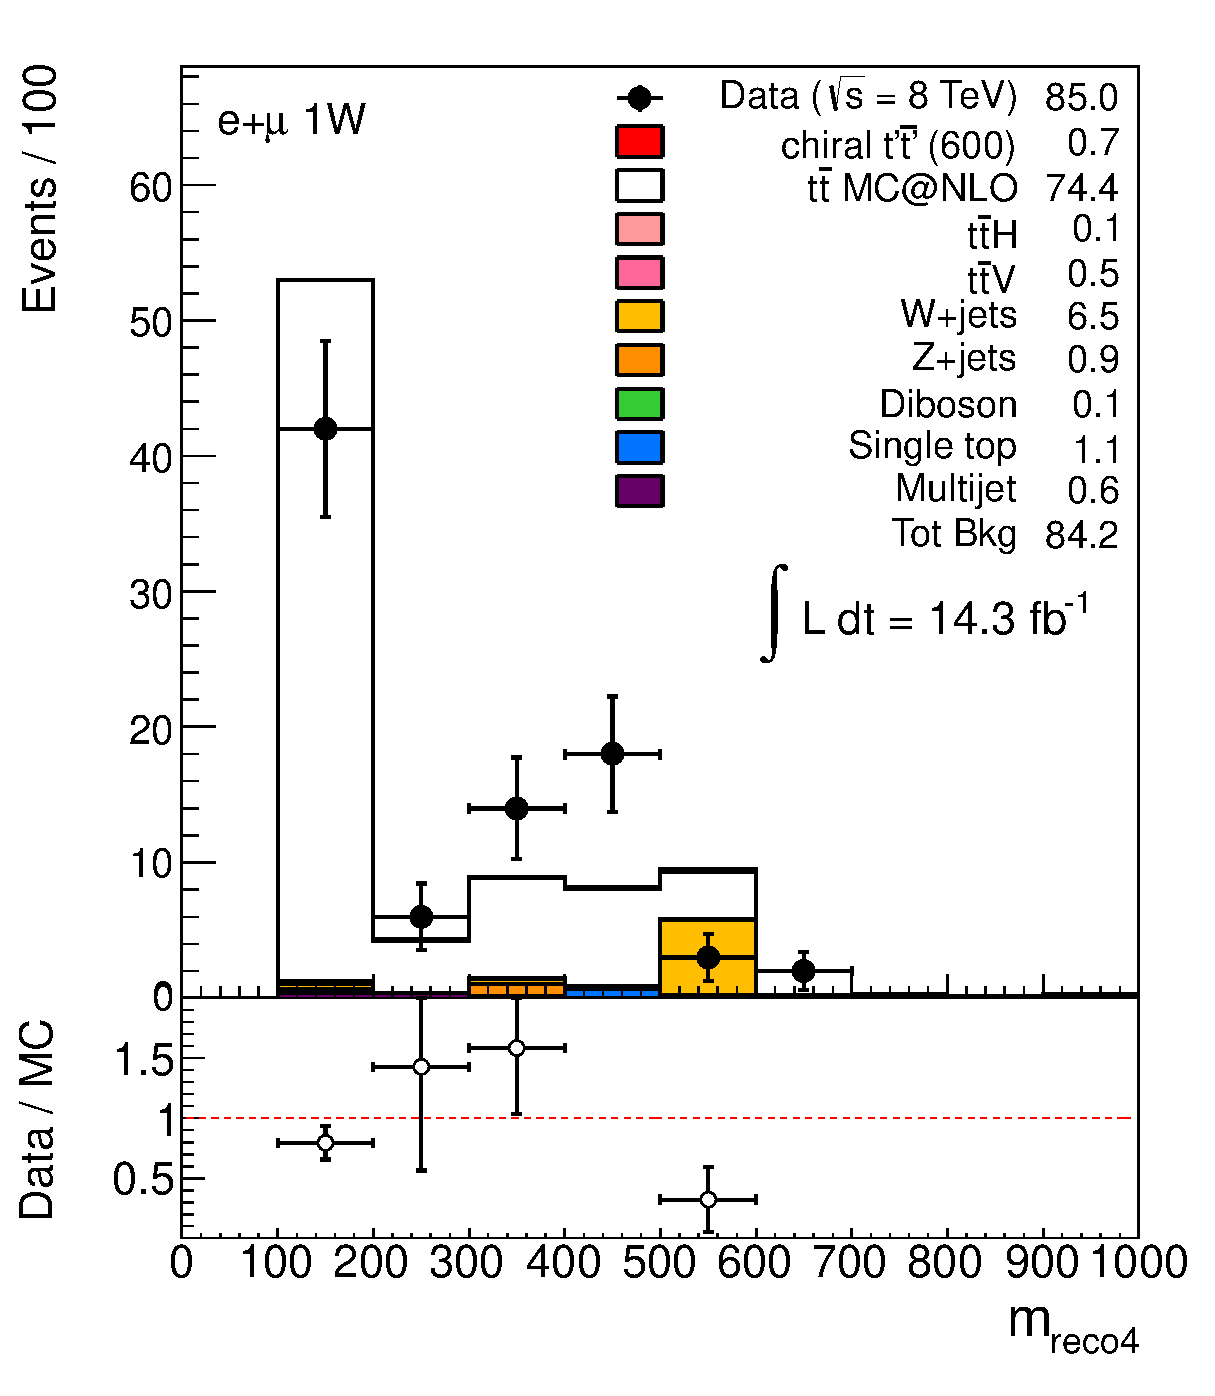
\includegraphics[width=0.3\textwidth]{appendices/figures/genmod/ttbar5200/VLQAna_WbX_1W_MWb_4_ELEMUONCR1_1W_NOMINAL.eps}}
}
\resizebox{1.5\textwidth}{!}{
	\subfigure[]{
          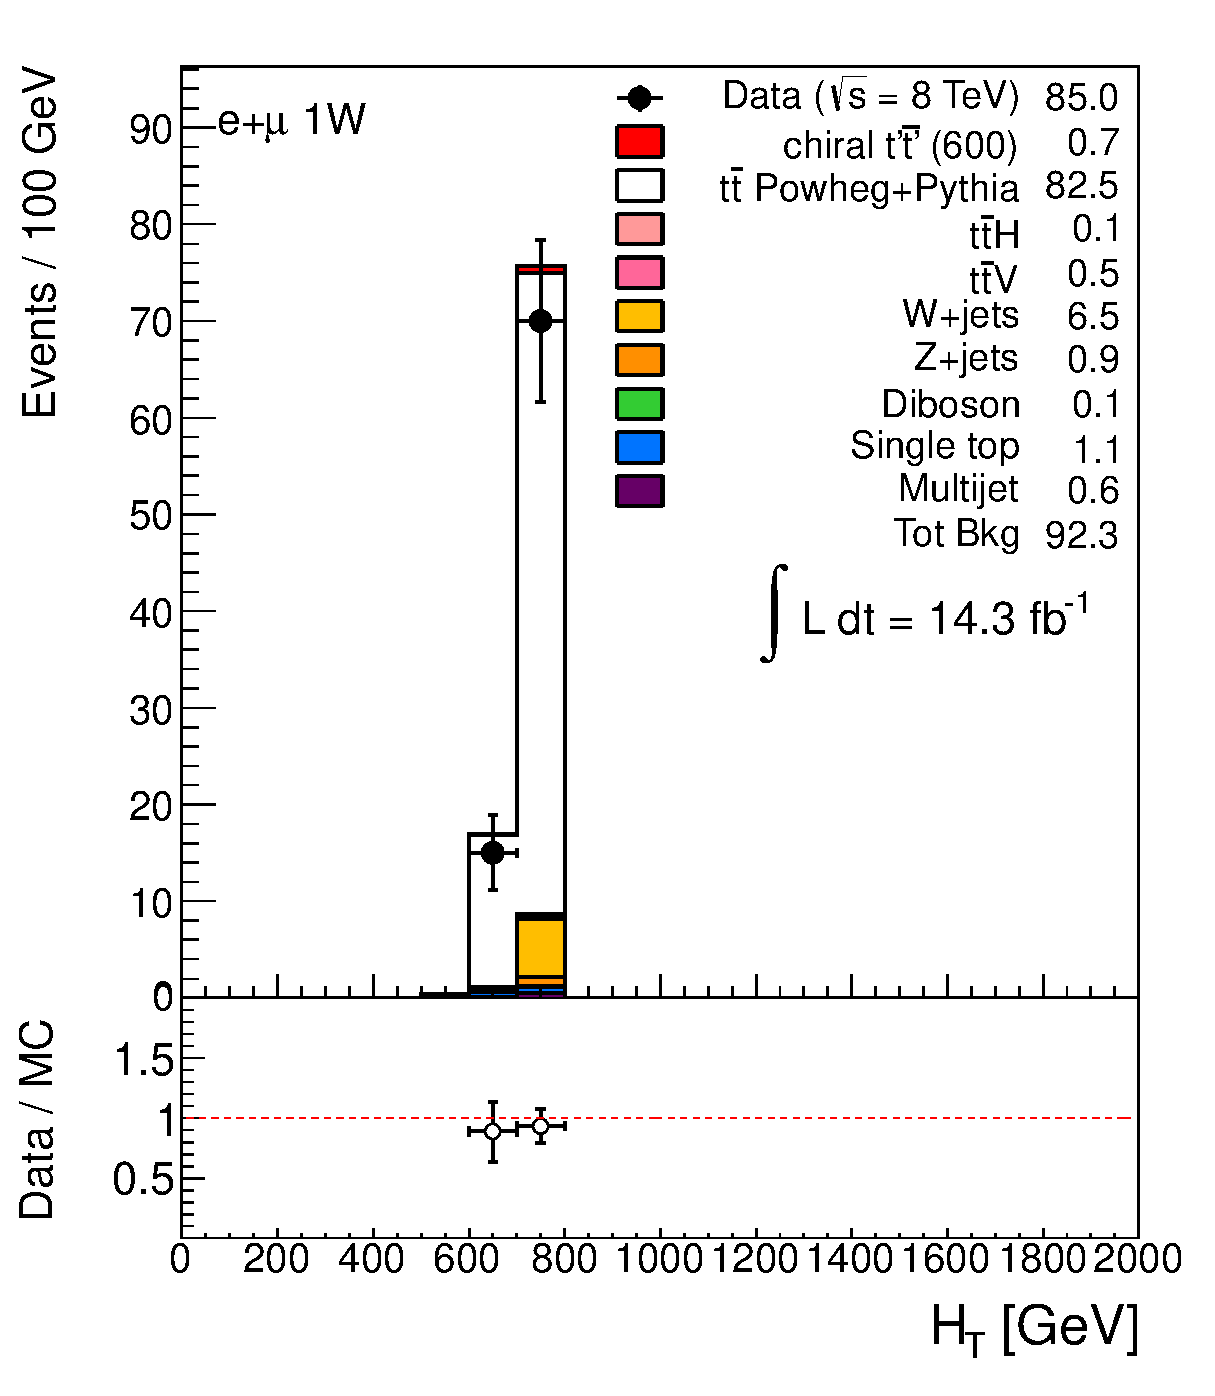
\includegraphics[width=0.3\textwidth]{appendices/figures/genmod/ttbar117050/HTAll_ELEMUONCR1_1W_NOMINAL.eps}}
	\subfigure[]{
          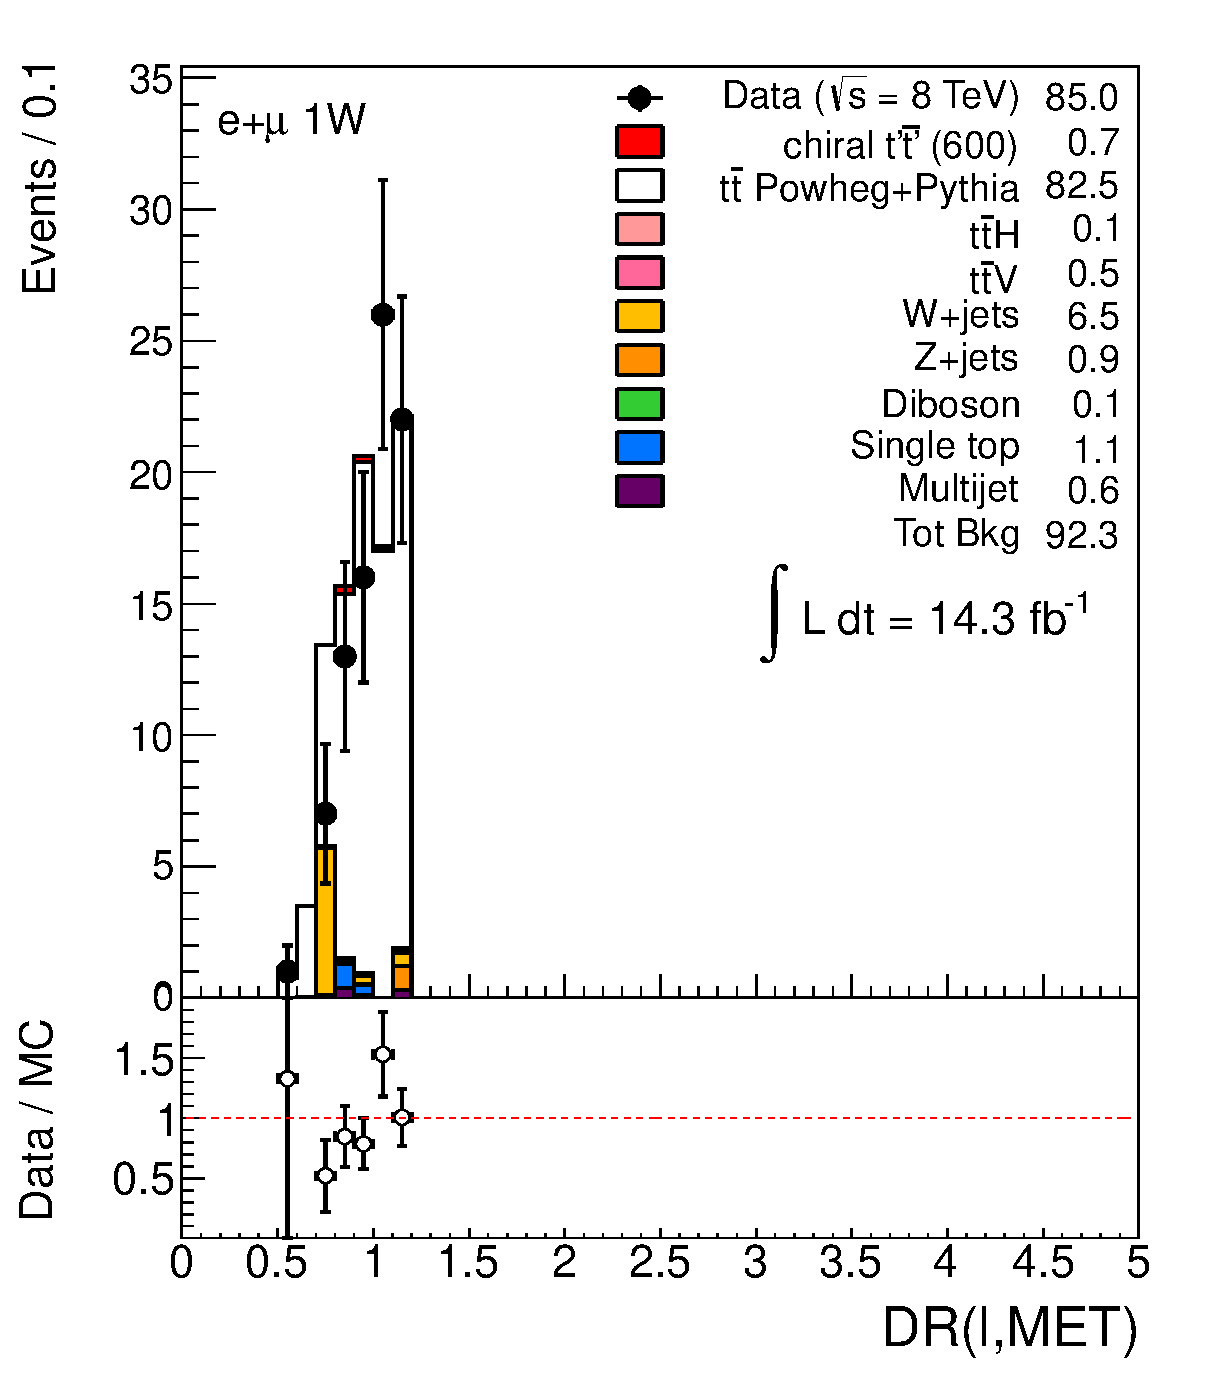
\includegraphics[width=0.3\textwidth]{appendices/figures/genmod/ttbar117050/VLQAna_WbX_DRLepMet_ELEMUONCR1_1W_NOMINAL.eps}}
	\subfigure[]{
          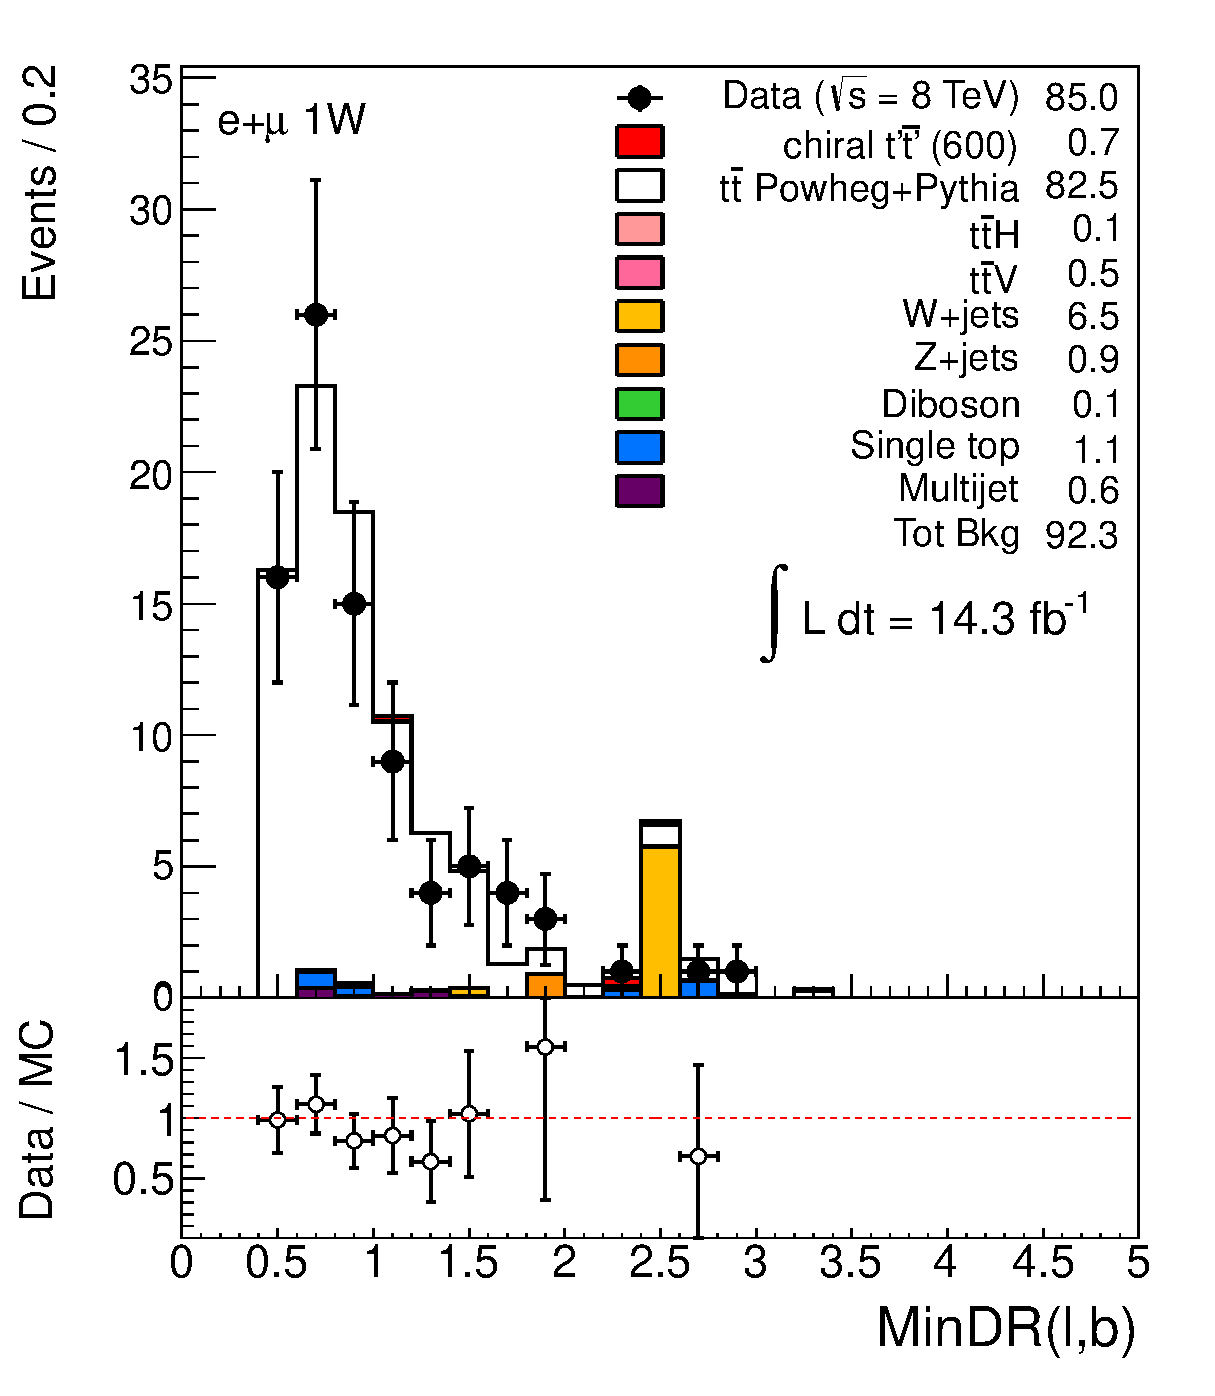
\includegraphics[width=0.3\textwidth]{appendices/figures/genmod/ttbar117050/VLQAna_WbX_MinDRlb_ELEMUONCR1_1W_NOMINAL.eps}}
	\subfigure[]{
          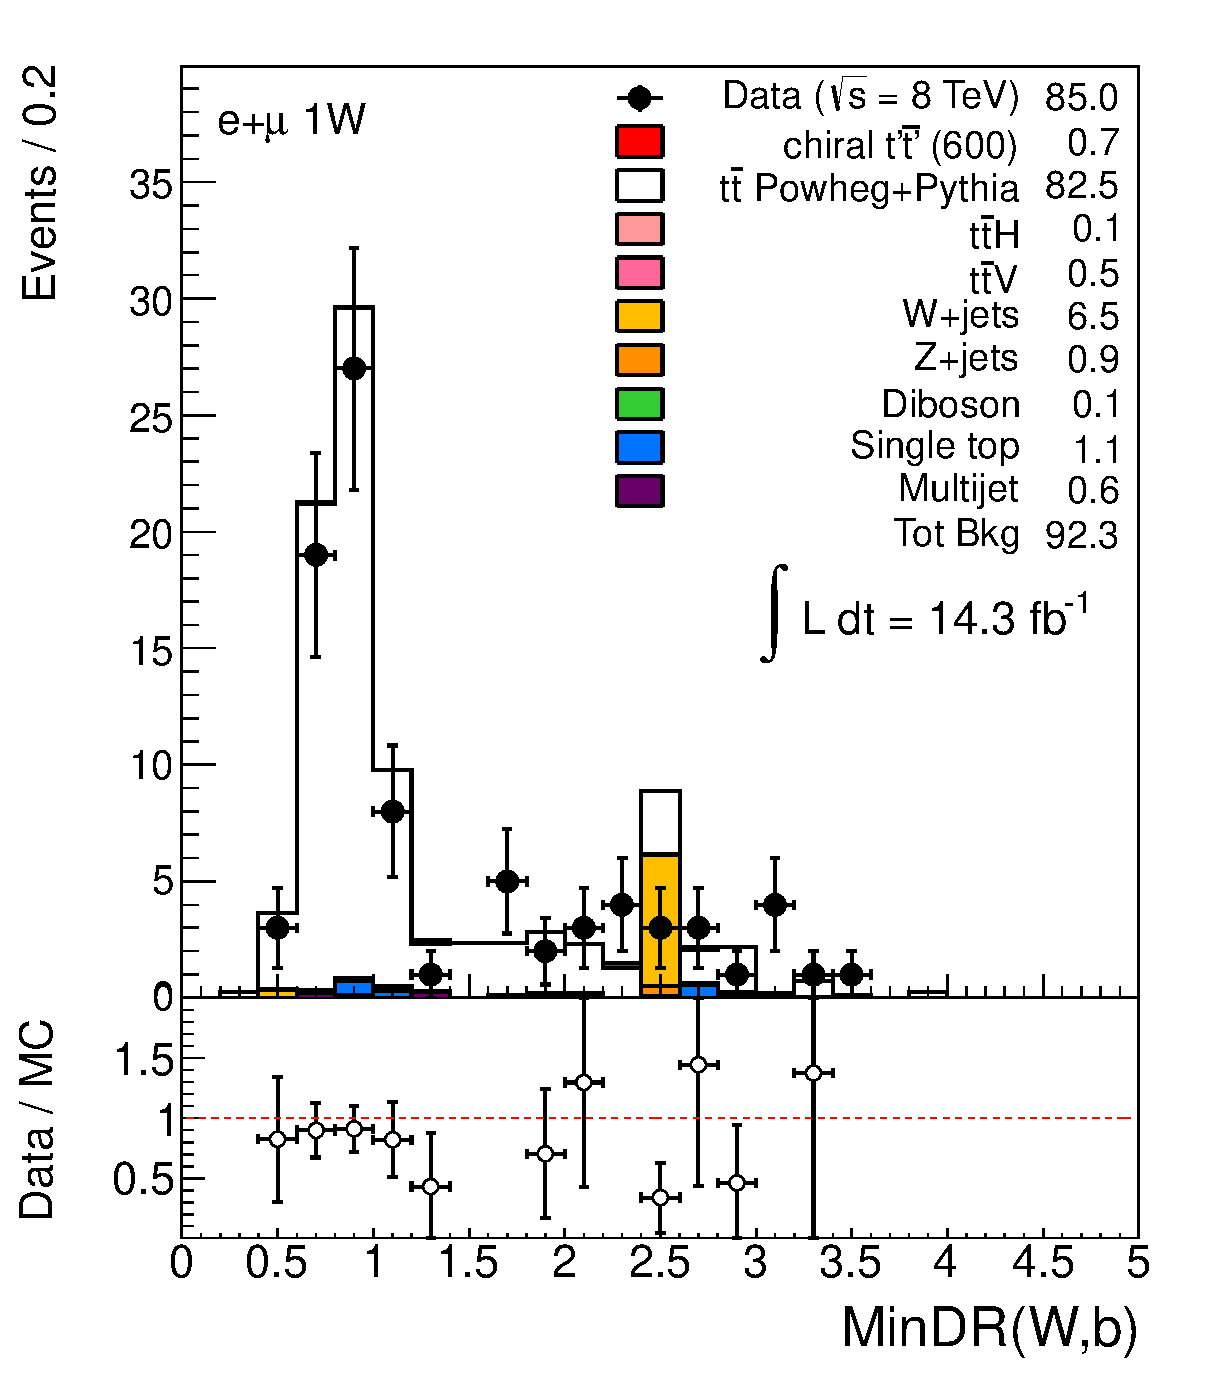
\includegraphics[width=0.3\textwidth]{appendices/figures/genmod/ttbar117050/VLQAna_WbX_MinDRWb_ELEMUONCR1_1W_NOMINAL.eps}}
	\subfigure[]{
          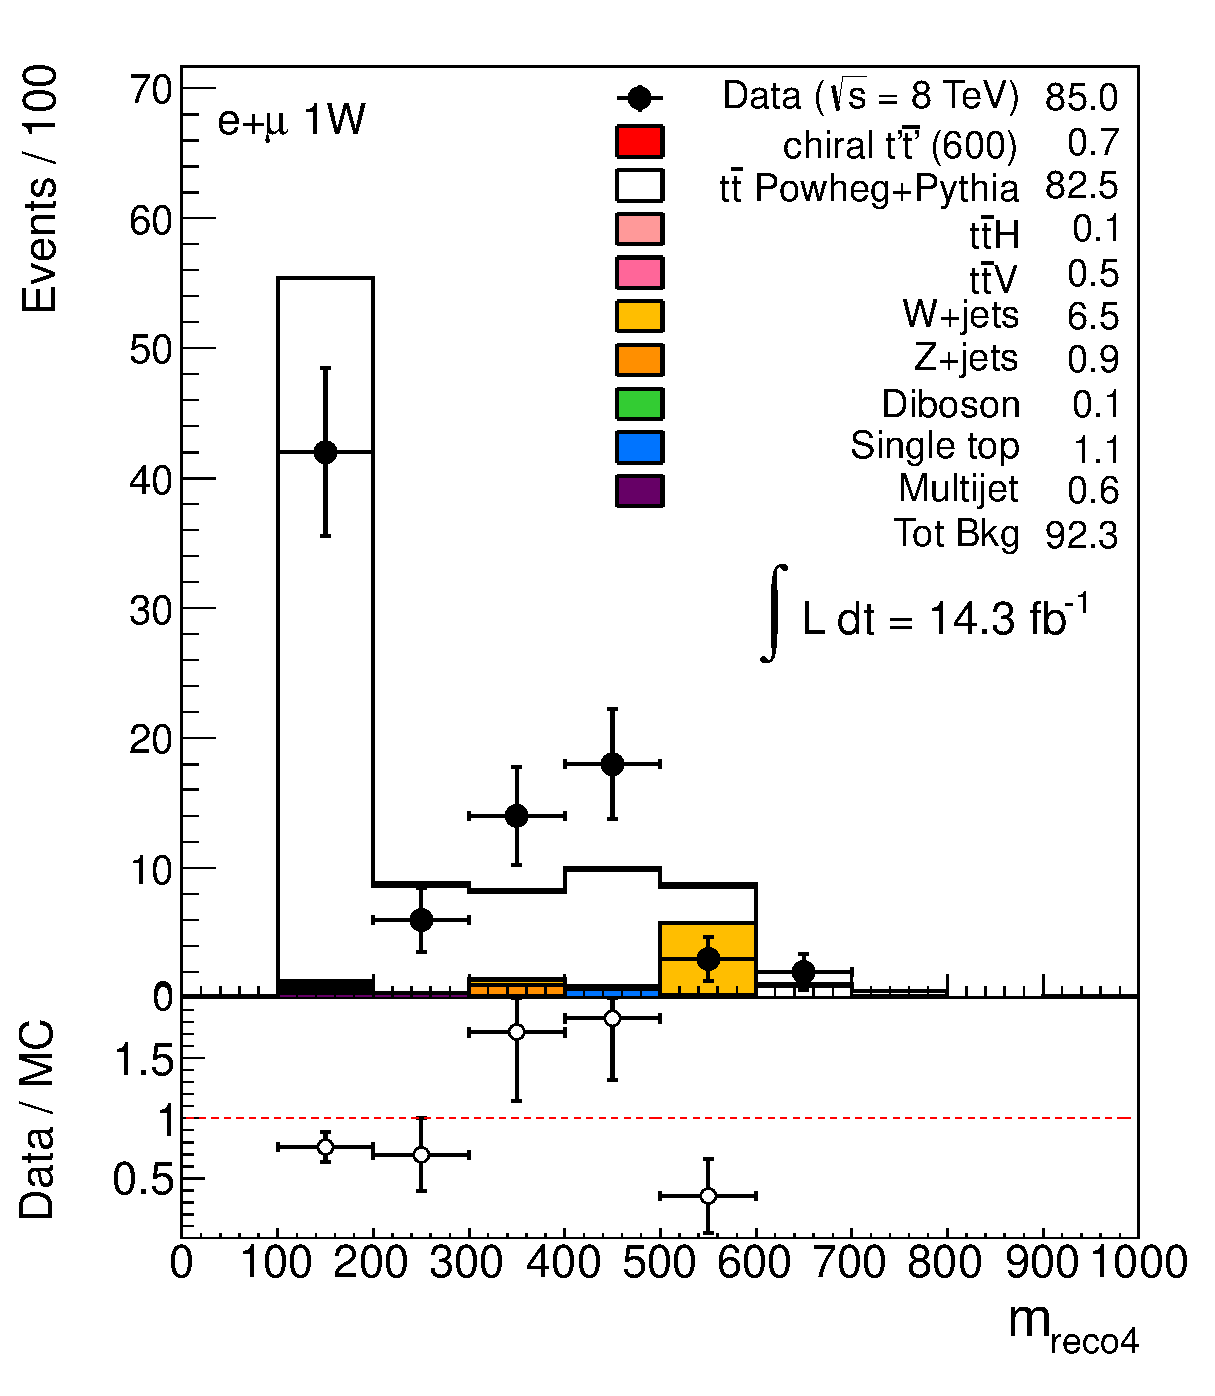
\includegraphics[width=0.3\textwidth]{appendices/figures/genmod/ttbar117050/VLQAna_WbX_1W_MWb_4_ELEMUONCR1_1W_NOMINAL.eps}}
}
\resizebox{1.5\textwidth}{!}{
	\subfigure[]{
          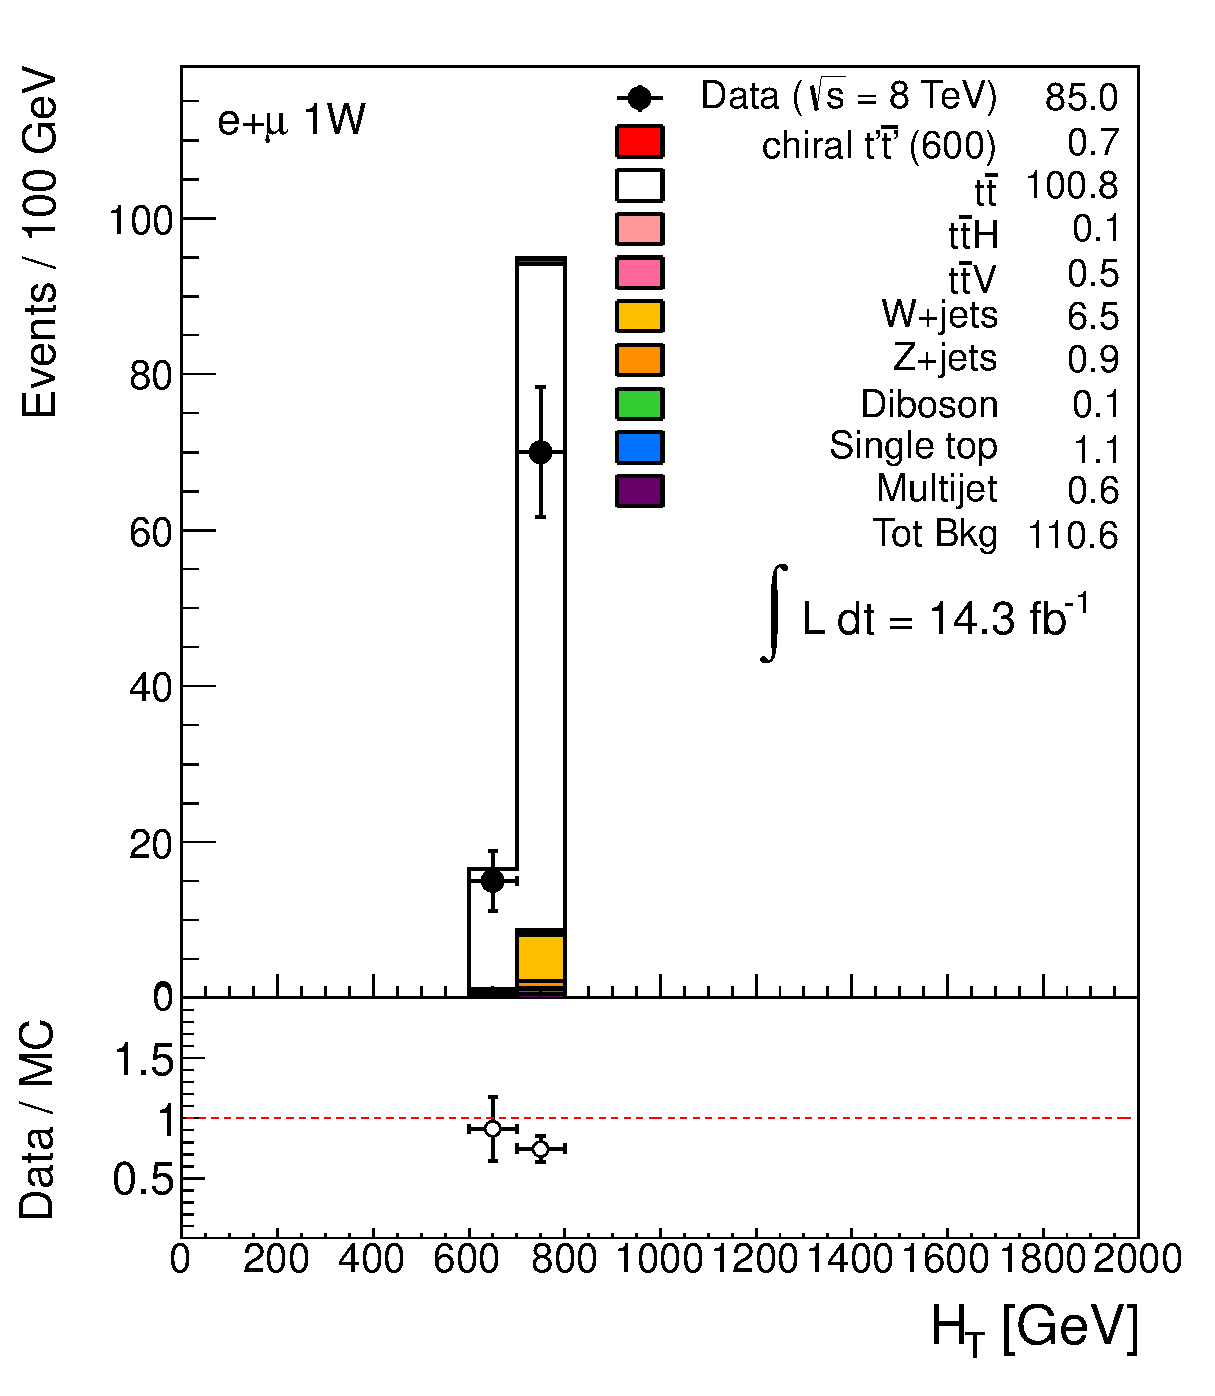
\includegraphics[width=0.3\textwidth]{appendices/figures/genmod/ttbarAlpgen_HFOR/HTAll_ELEMUONCR1_1W_NOMINAL.eps}}
	\subfigure[]{
          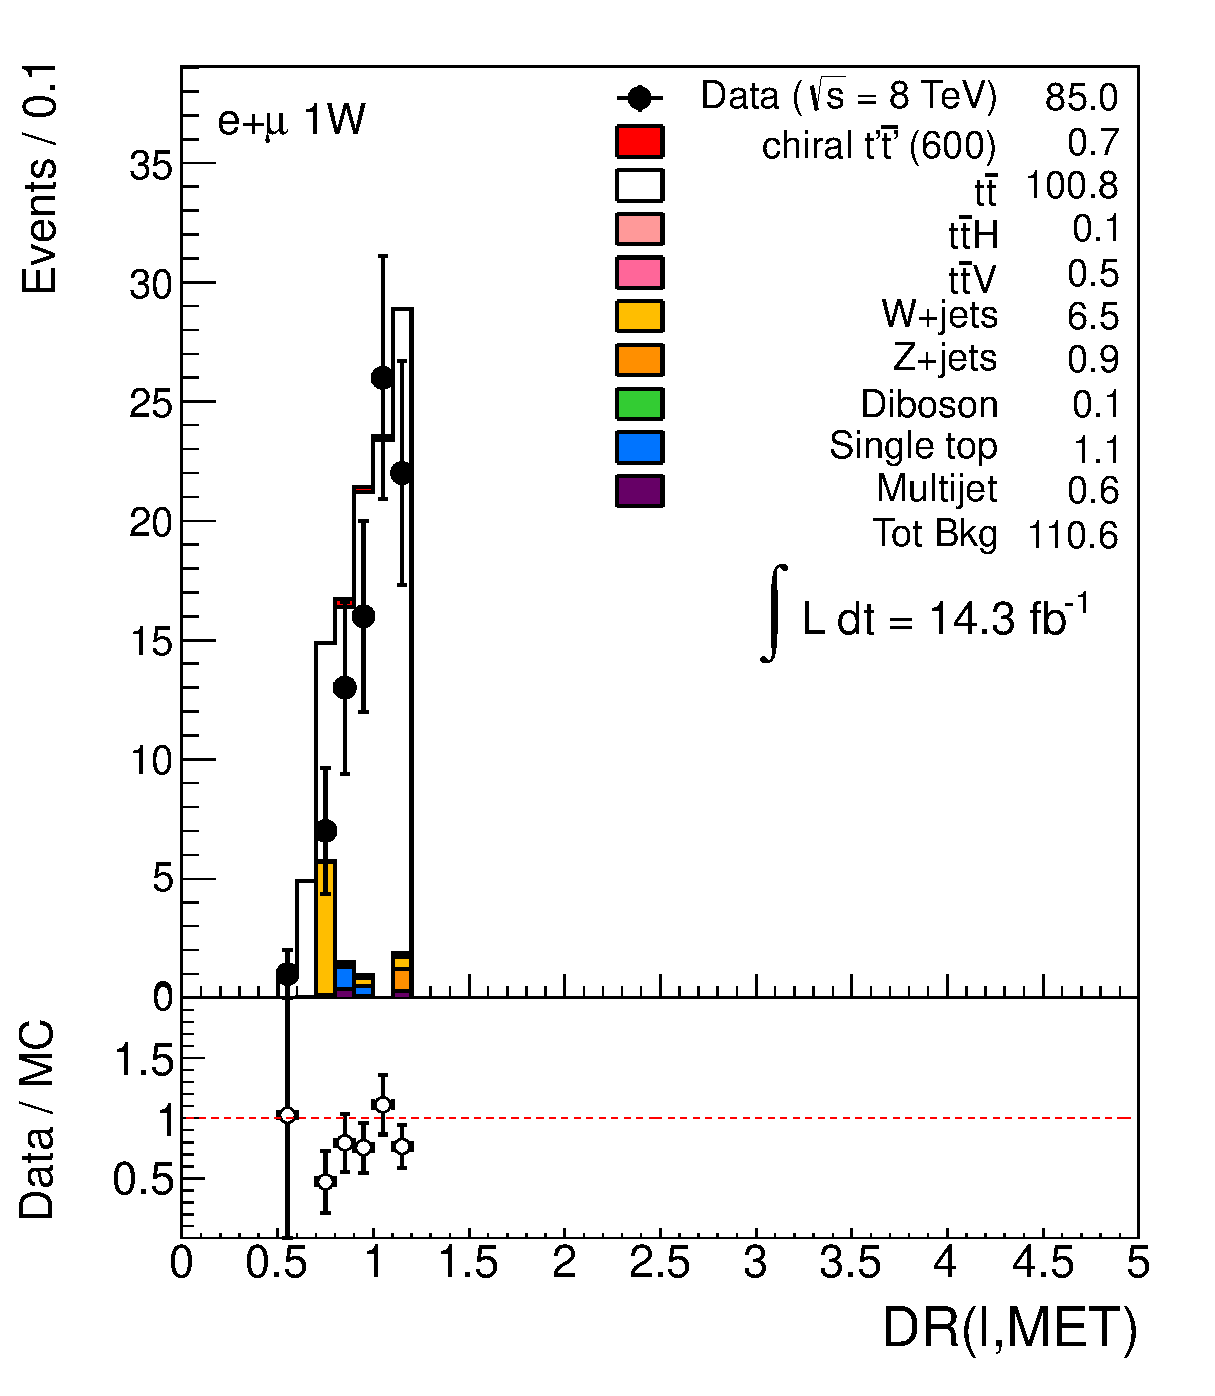
\includegraphics[width=0.3\textwidth]{appendices/figures/genmod/ttbarAlpgen_HFOR/VLQAna_WbX_DRLepMet_ELEMUONCR1_1W_NOMINAL.eps}}
	\subfigure[]{
          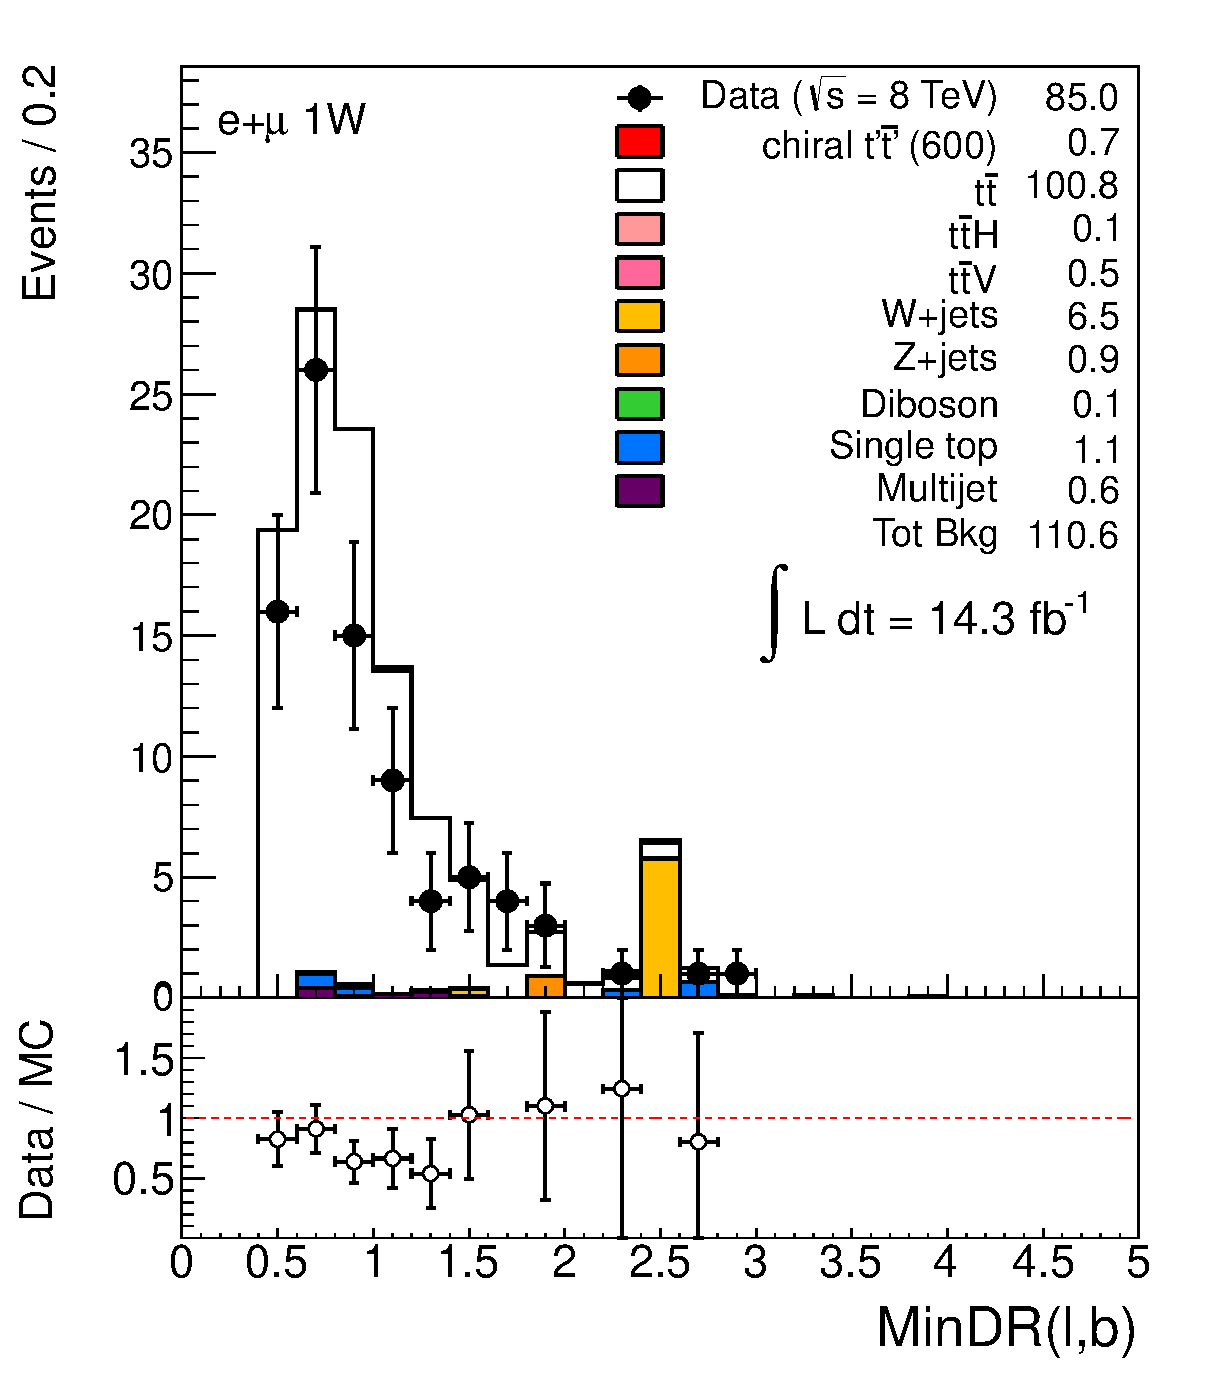
\includegraphics[width=0.3\textwidth]{appendices/figures/genmod/ttbarAlpgen_HFOR/VLQAna_WbX_MinDRlb_ELEMUONCR1_1W_NOMINAL.eps}}
	\subfigure[]{
          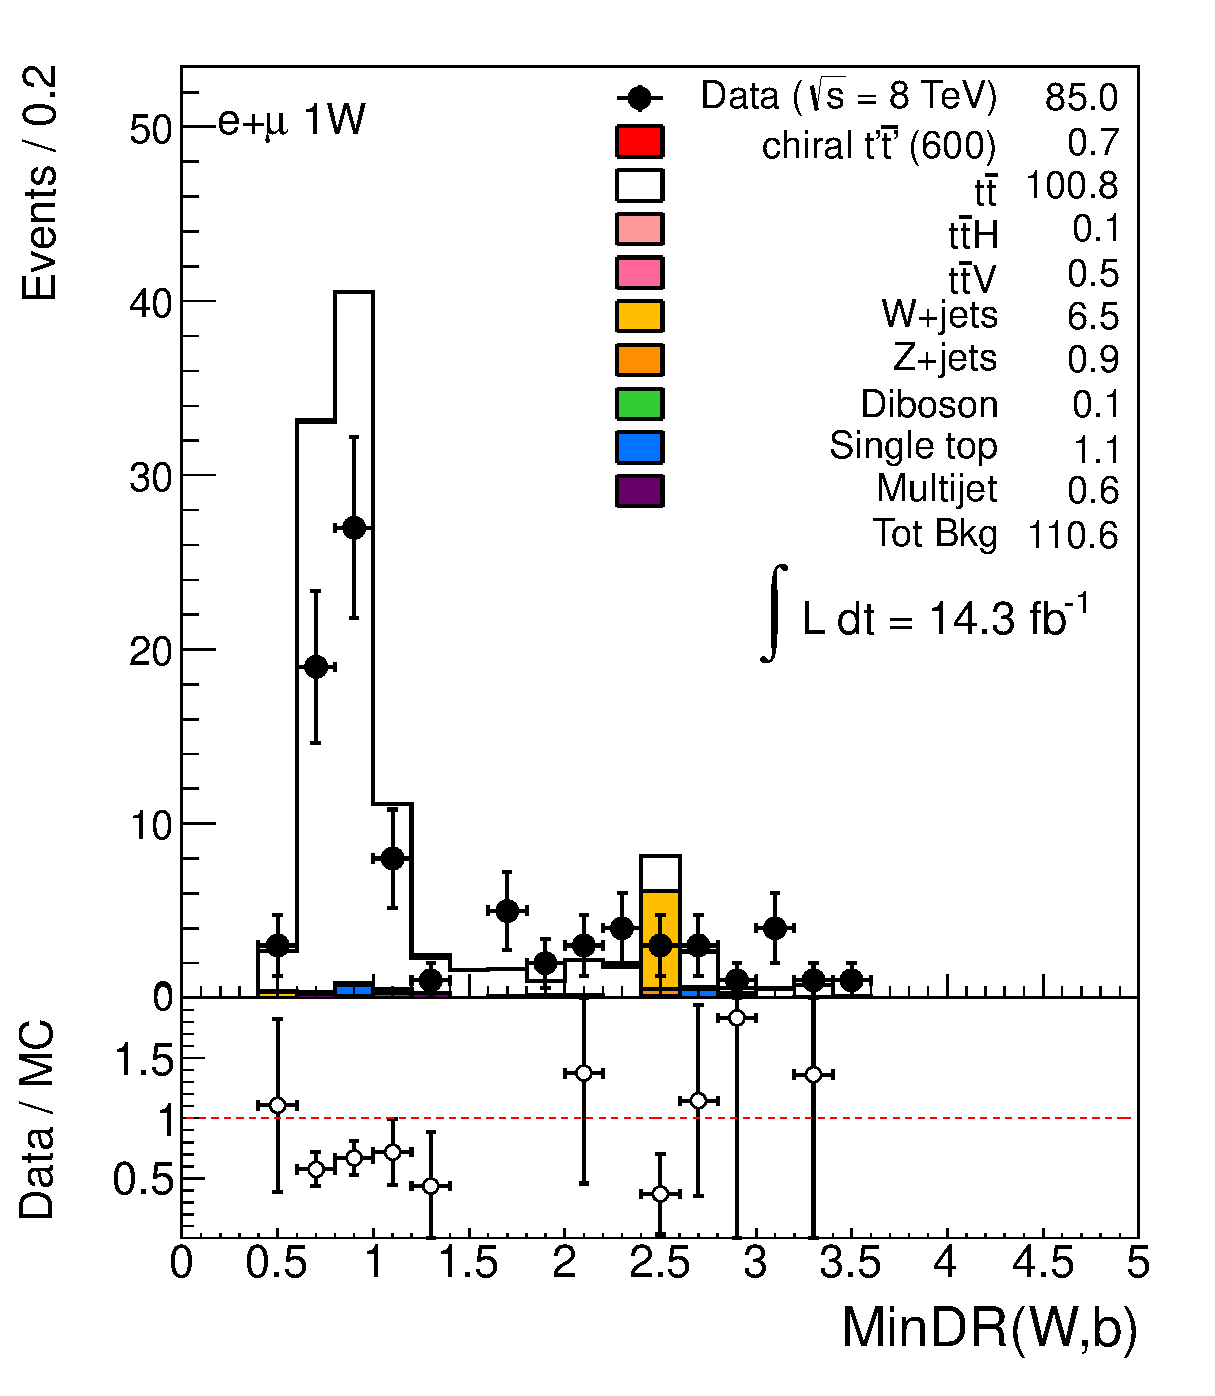
\includegraphics[width=0.3\textwidth]{appendices/figures/genmod/ttbarAlpgen_HFOR/VLQAna_WbX_MinDRWb_ELEMUONCR1_1W_NOMINAL.eps}}
	\subfigure[]{
          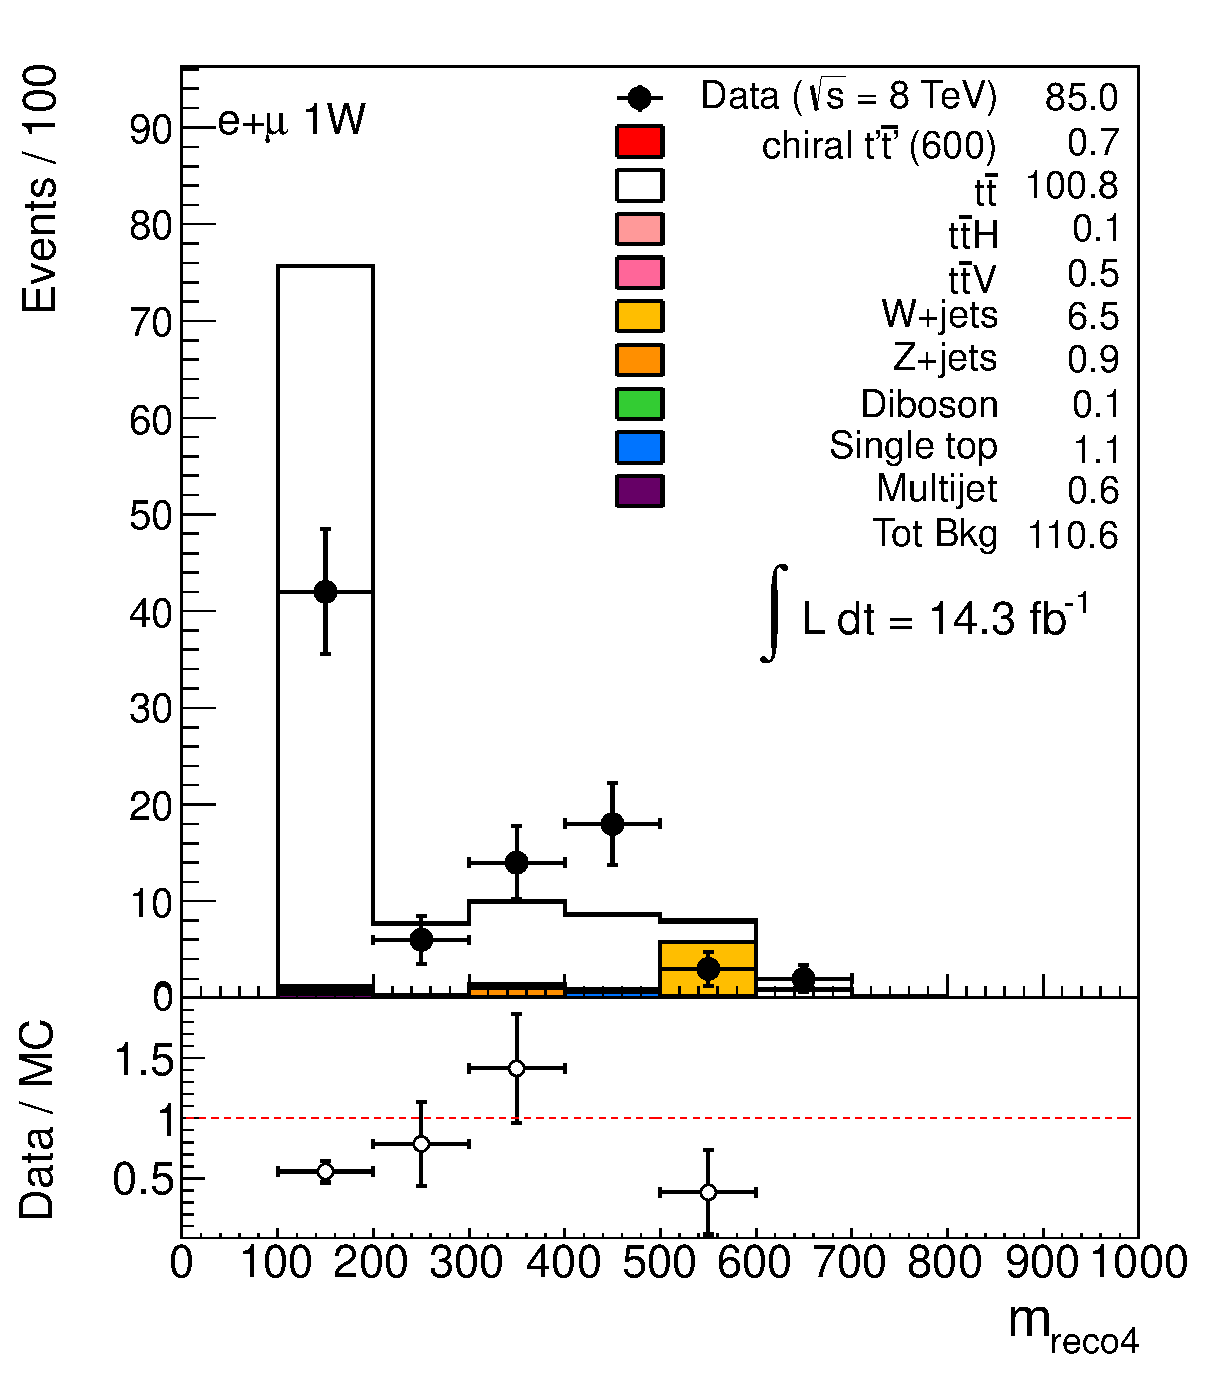
\includegraphics[width=0.3\textwidth]{appendices/figures/genmod/ttbarAlpgen_HFOR/VLQAna_WbX_1W_MWb_4_ELEMUONCR1_1W_NOMINAL.eps}}
}
	\caption{Comparison between data and prediction in the electron and muon combined channel in SDR2
          for, from left to right:
          $\HT$ variable, $\Delta R(\ell,\nu)$, $\min(\Delta R(\ell, b_{1,2}))$, 
          $\min(\Delta R(W_{\rm had}, b_{1,2}))$ and $m_{\rm reco}$.
          The \ttbar\ background is simulated with: (a-e) \texttt{MC@NLO}, (f-j) \texttt{POWHEG+PYTHIA},
          (k-o) \texttt{ALPGEN+HERWIG}. No systematic uncertainty is shown.\label{fig:genmodCR1}}
\end{center}\end{figure}
\end{landscape}
